\documentclass[fontsize=10pt]{article}
\usepackage[utf8]{inputenc}
\usepackage[T1]{fontenc}
\usepackage{graphicx} % handles figures
\usepackage[fleqn]{mathtools}
\usepackage{amsmath}
\usepackage{hyperref}
\usepackage{amssymb}
\usepackage{xcolor}

\title{\textbf{Mathématiques discrètes}\\ Solutions TP 10}
\date{}
\begin{document}
\maketitle

\section*{Exercice 1}
Voir solutions TP 8 et TP 9.

\section*{Exercice 2}
\begin{enumerate}
\item
Toutes les triangularisations possibles pour un carré.
\begin{figure}[hbtp]
\centering
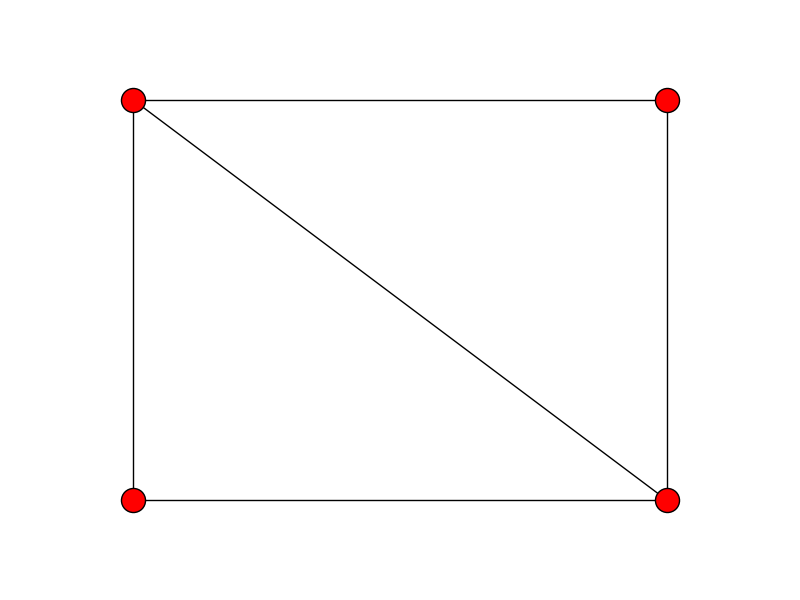
\includegraphics[scale=0.1]{imgs/carre/carre_1.png}
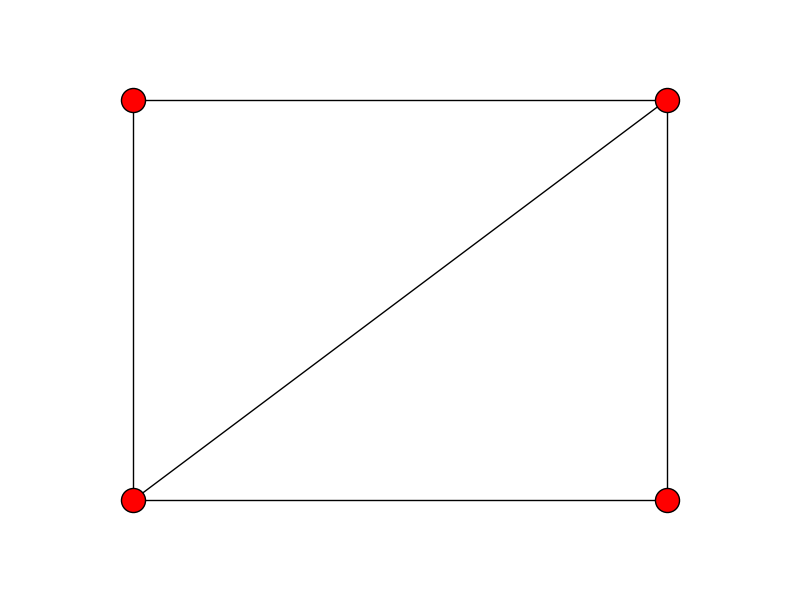
\includegraphics[scale=0.1]{imgs/carre/carre_2.png}
\end{figure}

Toutes les triangularisations possibles pour un pentagone.

\begin{figure}[hbtp]
\centering
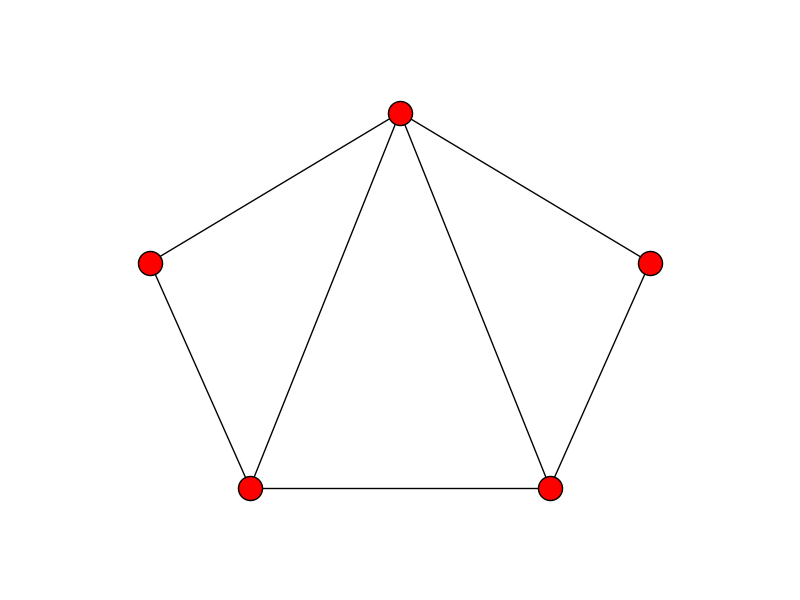
\includegraphics[scale=0.1]{imgs/pentagon/pentagon_1.png}
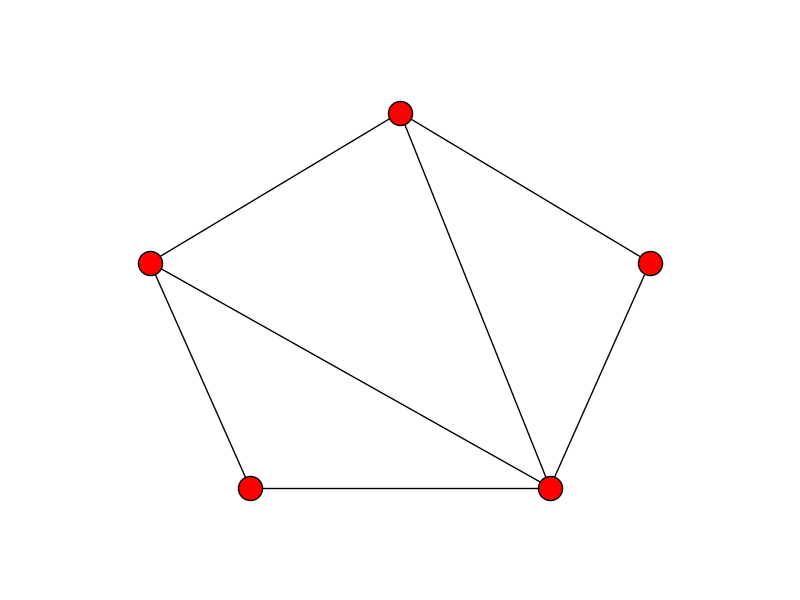
\includegraphics[scale=0.1]{imgs/pentagon/pentagon_2.png}
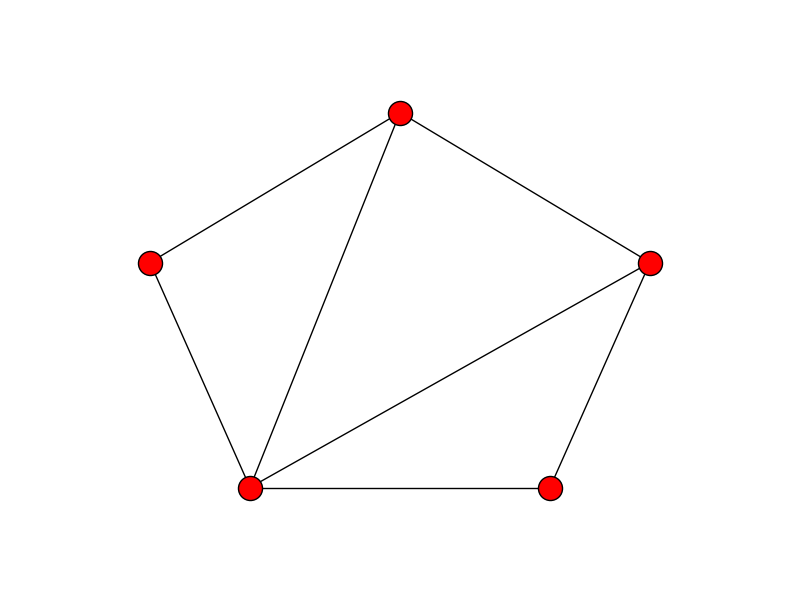
\includegraphics[scale=0.1]{imgs/pentagon/pentagon_3.png}
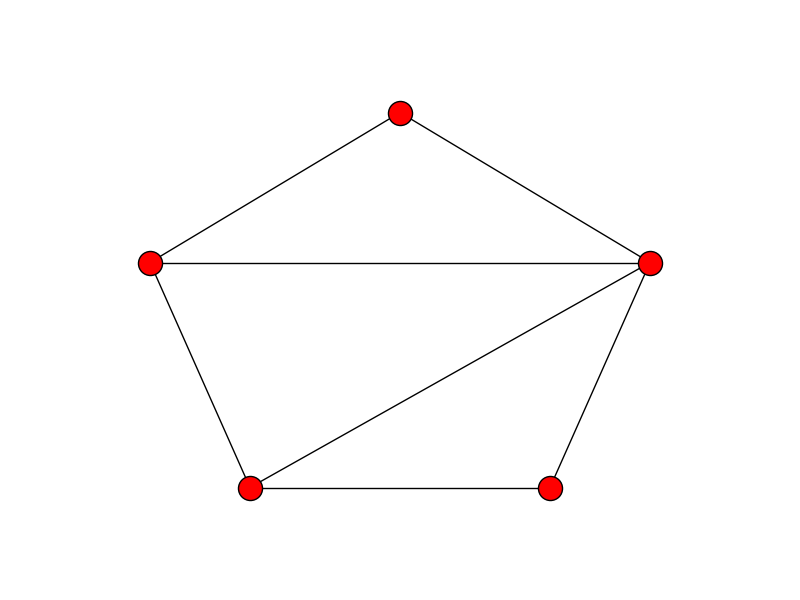
\includegraphics[scale=0.1]{imgs/pentagon/pentagon_4.png}
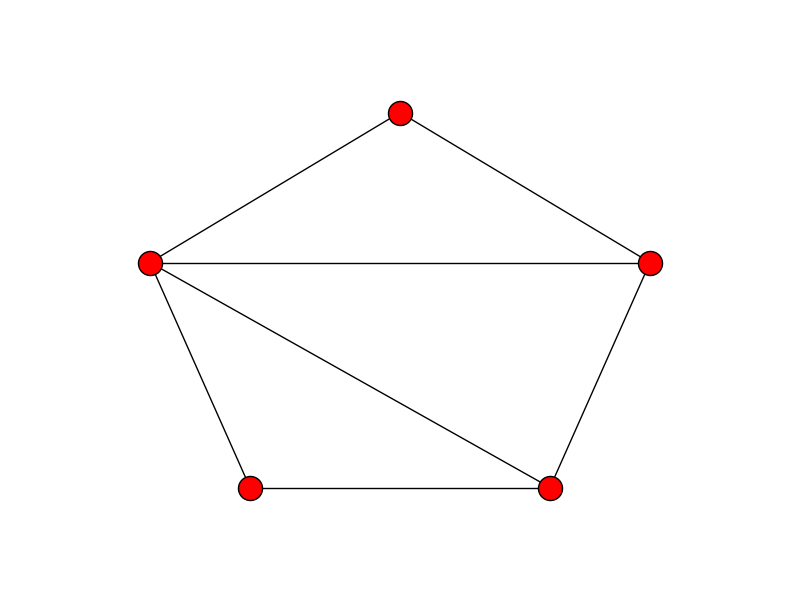
\includegraphics[scale=0.1]{imgs/pentagon/pentagon_5.png}
\end{figure}

Toutes les triangularisations possibles pour un hexagone.

\begin{figure}[hbtp]
\centering
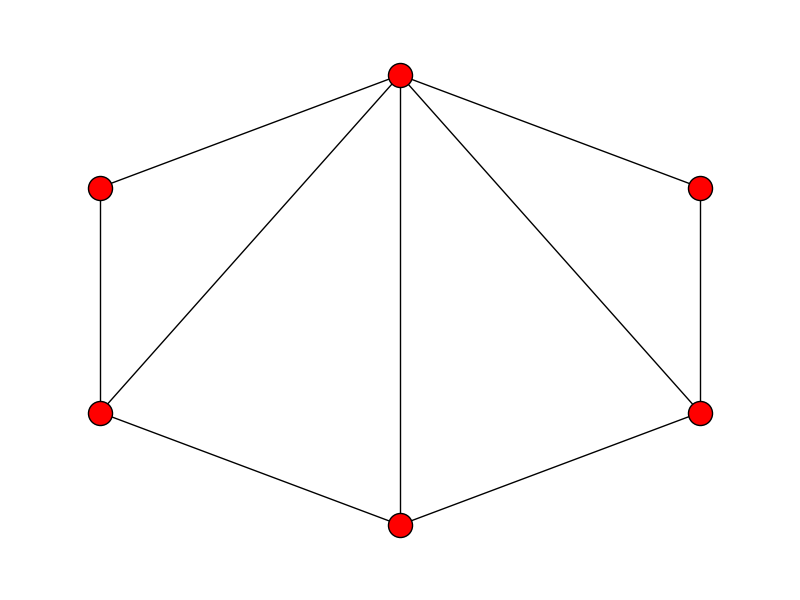
\includegraphics[scale=0.1]{imgs/hexagon/hexagon_1.png}
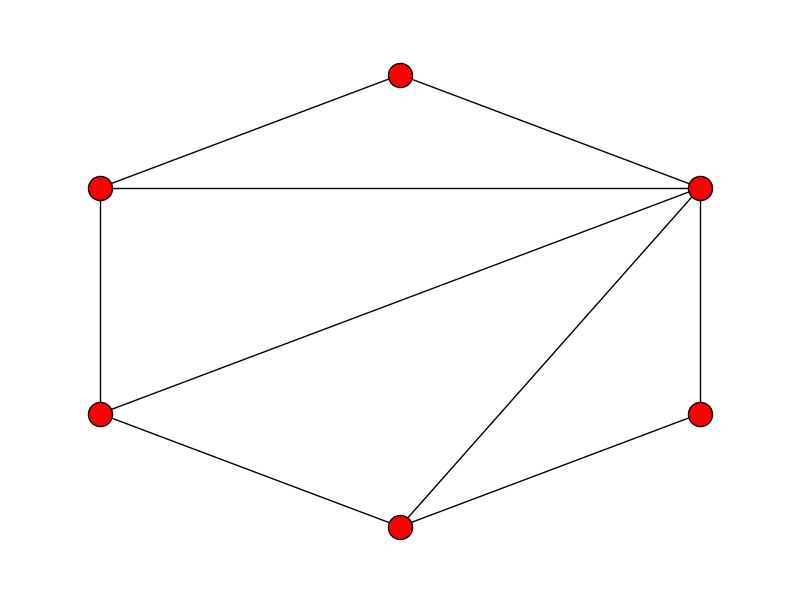
\includegraphics[scale=0.1]{imgs/hexagon/hexagon_2.png}
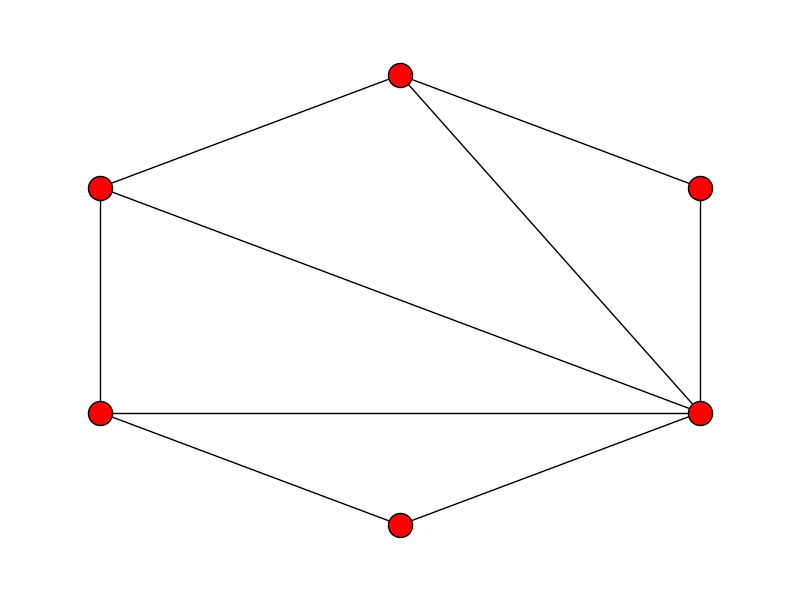
\includegraphics[scale=0.1]{imgs/hexagon/hexagon_3.png}
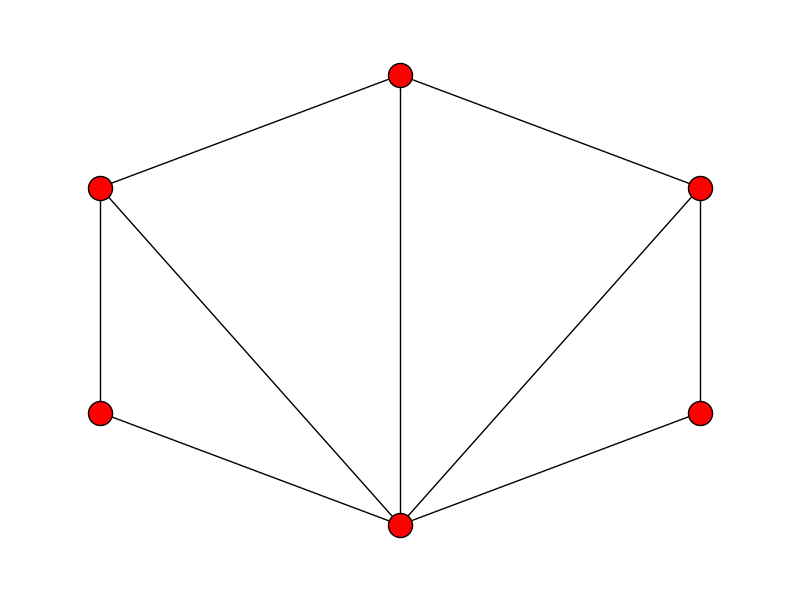
\includegraphics[scale=0.1]{imgs/hexagon/hexagon_4.png}
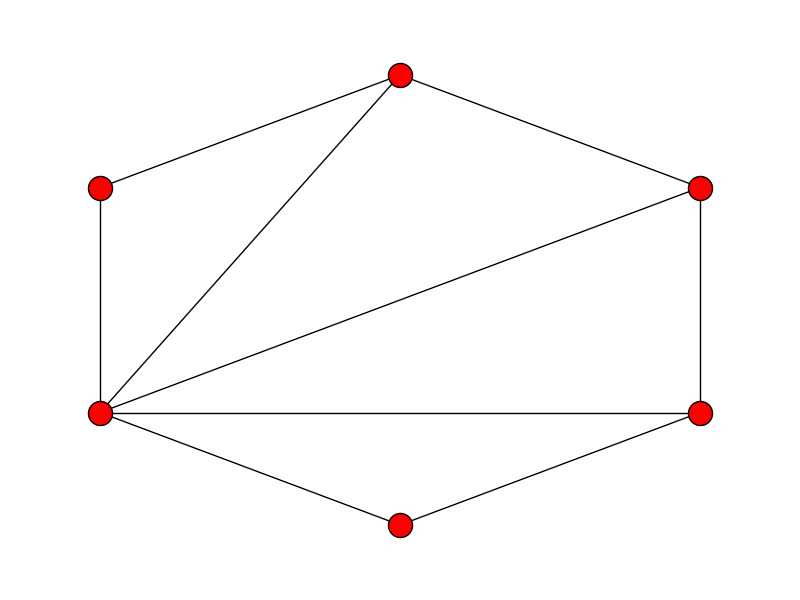
\includegraphics[scale=0.1]{imgs/hexagon/hexagon_5.png}
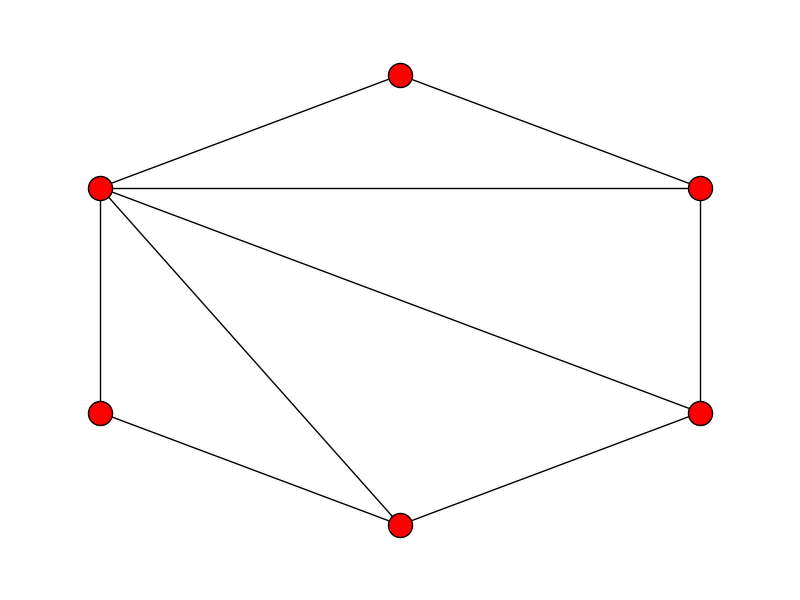
\includegraphics[scale=0.1]{imgs/hexagon/hexagon_6.png}
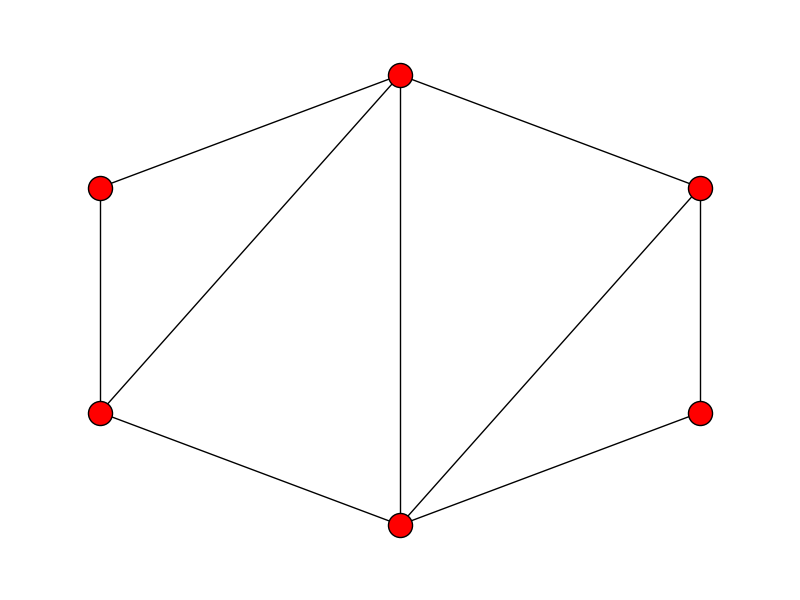
\includegraphics[scale=0.1]{imgs/hexagon/hexagon_7.png}
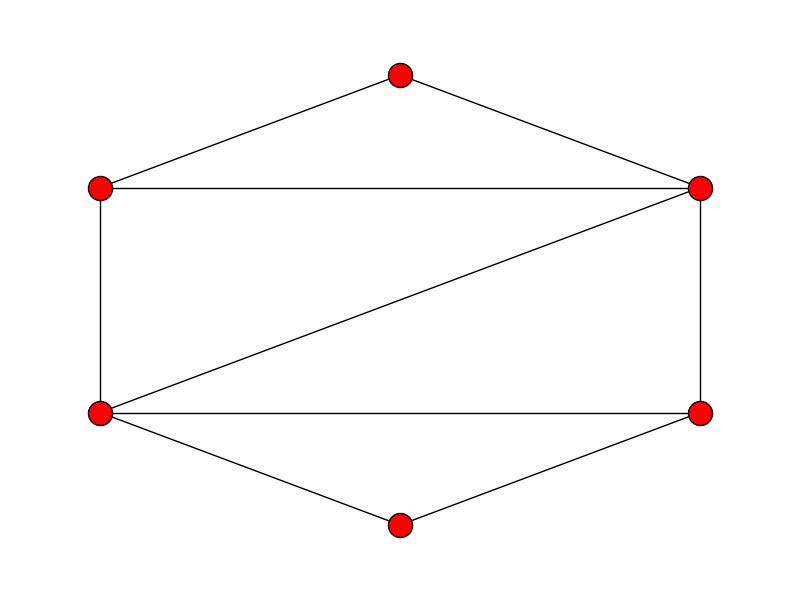
\includegraphics[scale=0.1]{imgs/hexagon/hexagon_8.png}
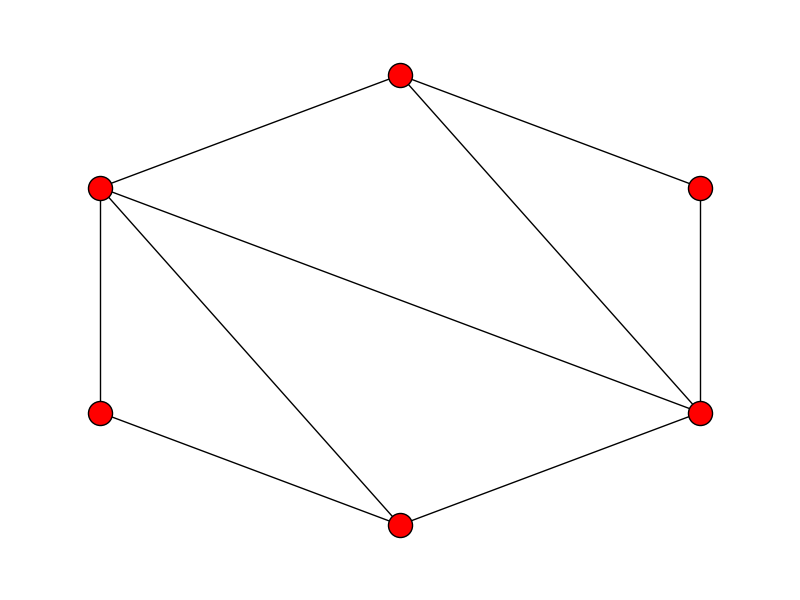
\includegraphics[scale=0.1]{imgs/hexagon/hexagon_9.png}
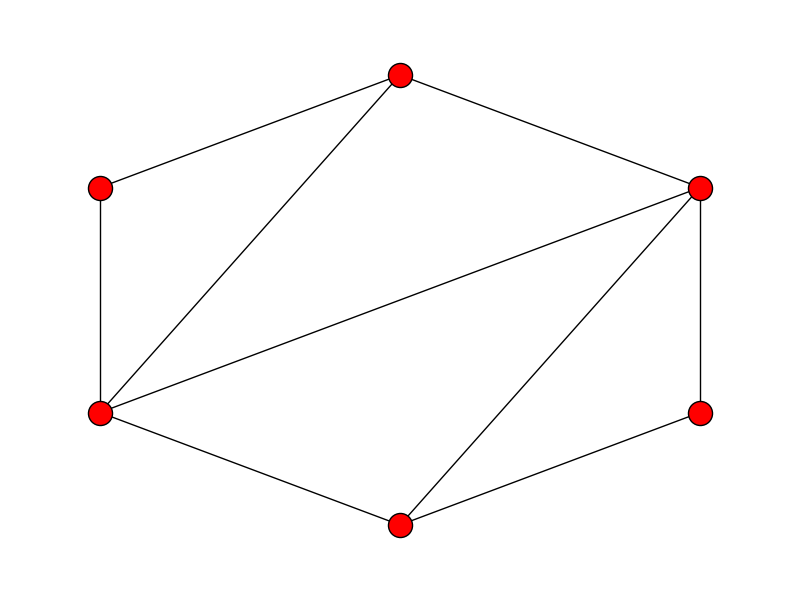
\includegraphics[scale=0.1]{imgs/hexagon/hexagon_10.png}
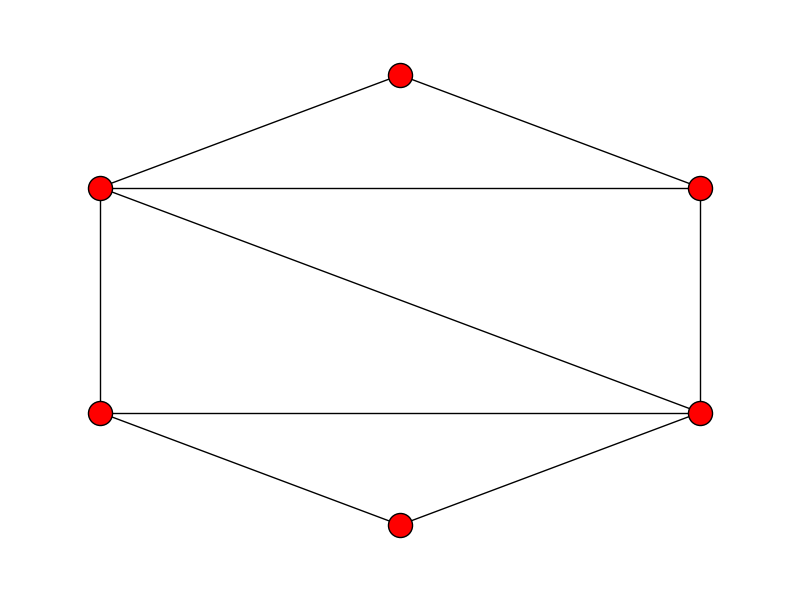
\includegraphics[scale=0.1]{imgs/hexagon/hexagon_11.png}
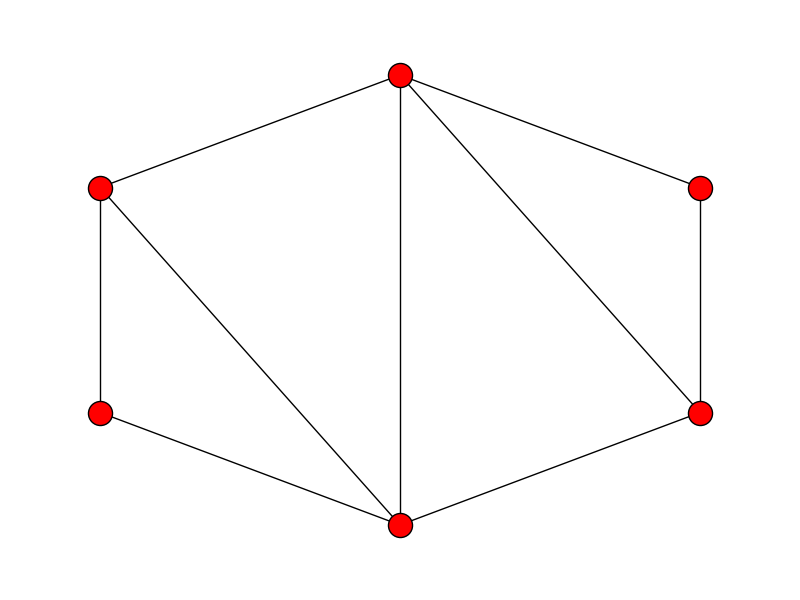
\includegraphics[scale=0.1]{imgs/hexagon/hexagon_12.png}
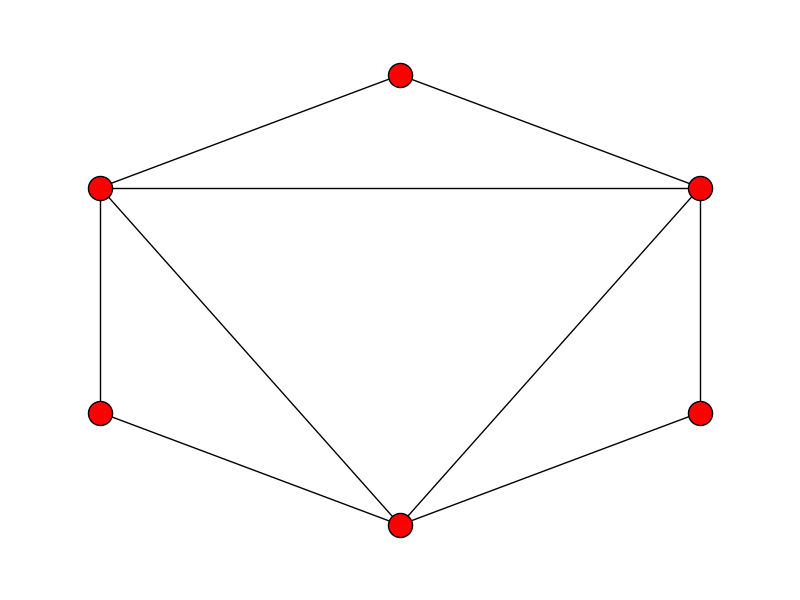
\includegraphics[scale=0.1]{imgs/hexagon/hexagon_13.png}
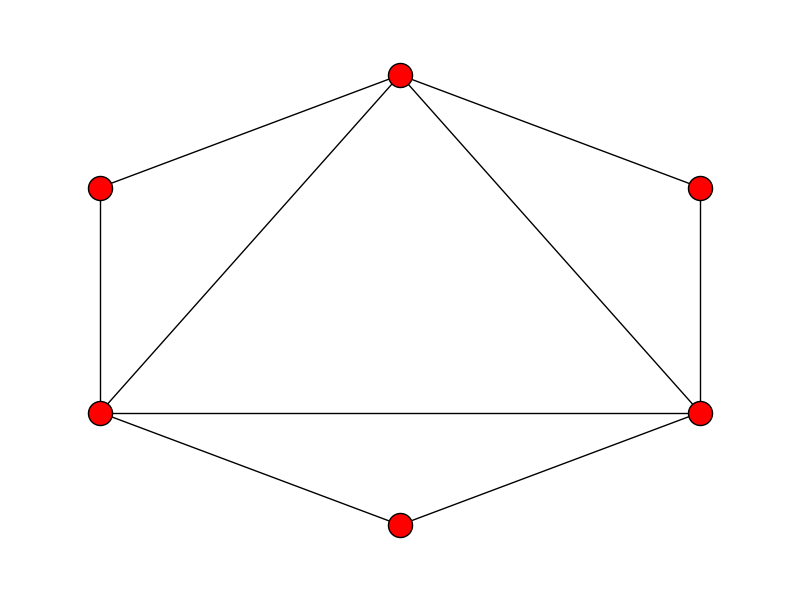
\includegraphics[scale=0.1]{imgs/hexagon/hexagon_14.png}
\end{figure}

\item C'est une récurrence, car la première triangularisation réduit le polygone en 2 polygones inférieurs.\\
Pour $T_n$, le nombre de façons de triangulariser un n-gone:\\ 
\begin{align*}
& T_n = \sum^{n-2}_{i=0} T_{1+i} \phantom{a}T_{n-1-i}
\end{align*}
\end{enumerate}

\section*{Exercice 3}
Pour toute montée, on ouvre une paranthèse. \newline
Pour tout plat, on ferme une paranthèse.

\end{document}
